\documentclass{beamer}
\usepackage{amsmath}
\usepackage{rotating}
\usepackage{graphicx}
\usepackage{multimedia}

\useinnertheme[shadow=true]{rounded}
\useoutertheme{shadow}
\usecolortheme{orchid}
\usecolortheme{whale}

\mode<presentation>

\newcommand{\dif}{\, \mathrm{d}}
\newcommand{\diff}[2]{\frac{\mathrm{d}#1}{\mathrm{d}#2}}
\newcommand{\partdiff}[2]{\frac{\partial #1}{\partial #2}}


\title{TMA4280 - Introduction to supercomputing}
\subtitle{Multi processor systems}
\author{Einar M. R{\o}nquist \and Arne Morten Kvarving}
\institute{NTNU \and Sintef ICT}
\date{January, 2010, revised January 2012}

\begin{document}

\maketitle

\begin{frame}\frametitle{Recent supercomputers at NTNU}

\begin{tabular}{|l|l|l|l|l|l|}
\hline
Year & System & \#proc & type & GF (*)\\
\hline
2000-2001 & SGI O2 & 160 & CCNUMA & 100\\
2001-2008 & SGI O3 & 898 & CCNUMA & 1000\\
2006-2011 & IBM P5+ & 2976 & distributed SMP & 23500\\
2012-     & SGI Altix ICE X & 23040 & distributed SMP & 497230 \\
\hline
\end{tabular}
\end{frame}

\begin{frame}\frametitle{Supercomputers}

\begin{itemize}
\item 70's - 80's: vector processors; \\
one or a few expensive, custom-made chips.
\vspace{.2cm}
\item 80's--: MPP systems; \\
many processors; standard micro-processors.
\vspace{.2cm}
\item Current trend: multicore systems; \\
heterogeneous computing. 
\end{itemize}
\end{frame}

\begin{frame}\frametitle{Multi-processor systems}
Challenges: 
\vspace{.5cm}

\begin{itemize}
\item communication between processors \\
(memory access, programming models); 
\vspace{.2cm}
\item computational methods or algorithms;
\vspace{.2cm}
\item scalability (hardware and algorithms); 
\vspace{.2cm}
\item large volumes of data (storage and visualization). 
\end{itemize}
\end{frame}

\begin{frame}\frametitle{Multi-processor systems: shared memory access}
\begin{center}
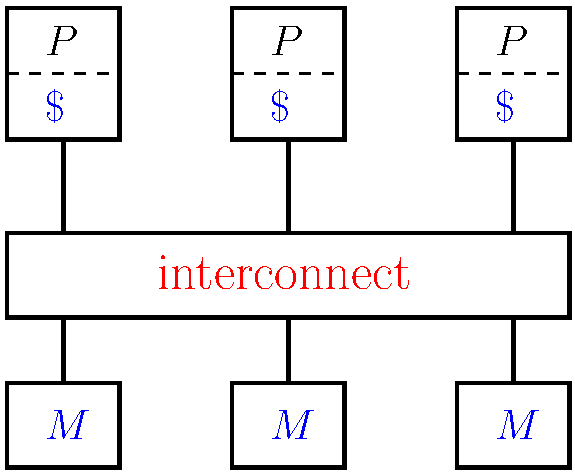
\includegraphics[width=7.5cm]{../../notes/03.multi/multiprocess1}
\end{center}
\end{frame}

\begin{frame}\frametitle{Multi-processor systems: distributed memory access}
\begin{center}
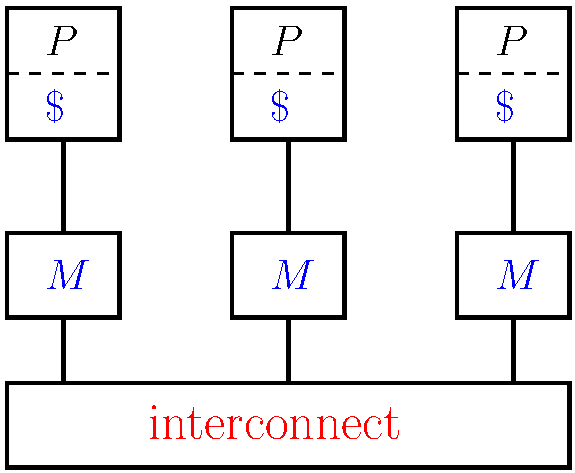
\includegraphics[width=7.5cm]{../../notes/03.multi/multiprocess2}
\end{center}
\end{frame}

\begin{frame}\frametitle{Shared memory systems: uniform memory access}
\begin{itemize}
\item Symmetric Multi-Processor (SMP); 
\item Examples: bus-based, switch-based, \textcolor{red}{crossbar} organizations.
\end{itemize}
\vspace{.2cm}
\begin{center}
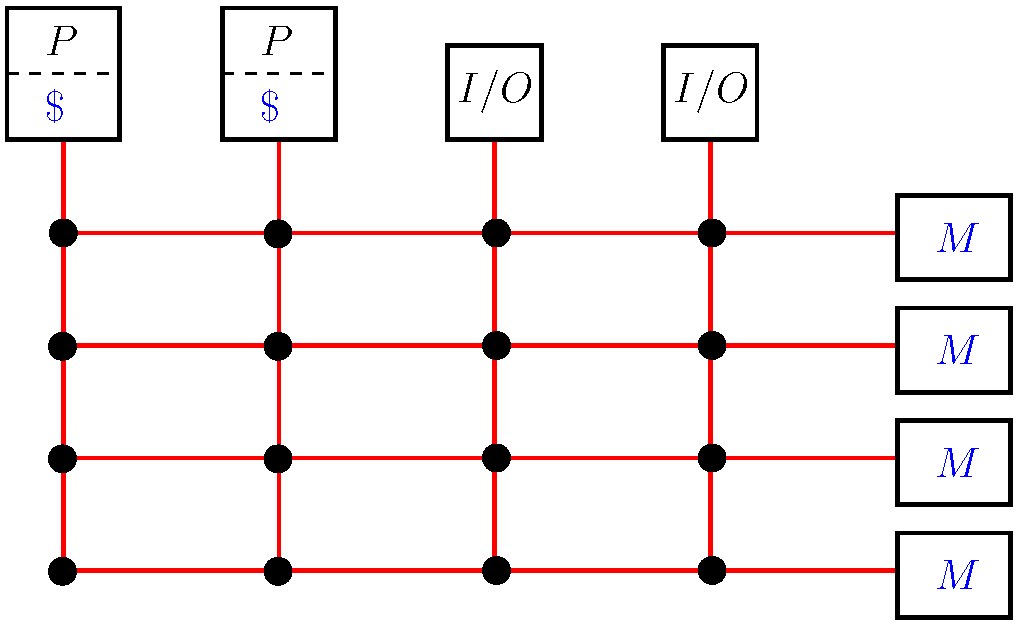
\includegraphics[width=7.5cm]{../../notes/03.multi/crossbar}
\end{center}
Challenges: cache coherency and cost.
\end{frame}

\begin{frame}\frametitle{Shared memory systems: non-uniform memory access}
\begin{itemize}
\vspace{.2cm}
\item ccNUMA: cache coherent non-uniform memory access;
\vspace{.2cm}
\item Examples: Several symmetric multi-processors (SMPs) connected via a high-speed 
low-latency network. 
\end{itemize}
\vspace{.3cm}
\begin{center}
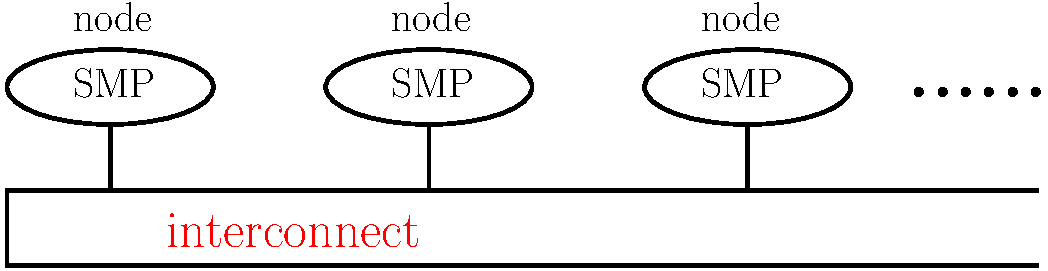
\includegraphics[width=8.5cm]{../../notes/03.multi/ccNUMA}
\end{center}
Each SMP (e.g., 16 processors) have uniform memory access. 
\end{frame}

\begin{frame}\frametitle{Distributed memory systems}
\begin{itemize}
\item Only the local address space is available to each processor;
\vspace{.2cm}
\item data from neighboring processors are only available through explicit 
message passing.
\end{itemize}
\vspace{.2cm}
\begin{center}
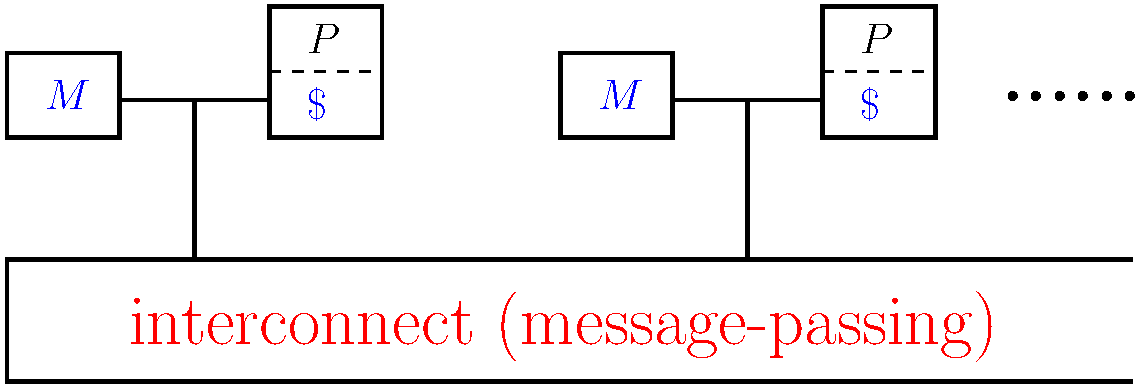
\includegraphics[width=8.5cm]{../../notes/03.multi/MIMD}
\end{center} 
\end{frame}

\begin{frame}\frametitle{Distributed memory systems: network topology}
Examples: 2D mesh / 2D toroid
\begin{center}
\begin{tabular}{lr}
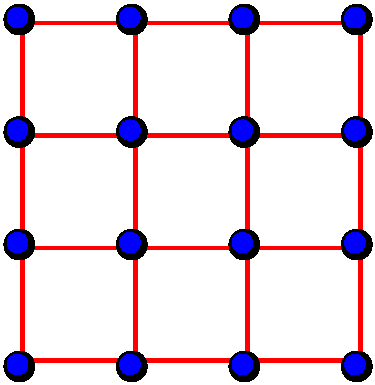
\includegraphics[width=3.5cm]{../../notes/03.multi/2Dmesh} \hspace{1.5cm}& \hspace{1.5cm}
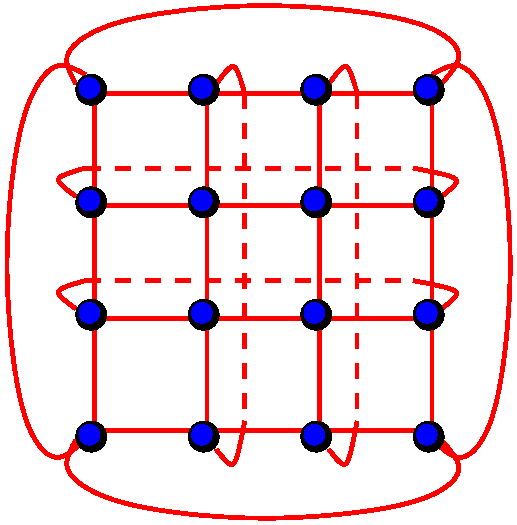
\includegraphics[width=4.cm]{../../notes/03.multi/2Dtoroid}
\end{tabular}
\end{center} 
Intel Paragon; Intel Delta (90's)\\
\vspace{1cm}
Other systems: 3D mesh (Cray T3D) and 3D toroid (Cray T3E)
Vilje: 8D enhanced hyper-cube.
\end{frame}

\begin{frame}\frametitle{The current supercomputer at NTNU}
Based on the Intel Sandy Bridge microprocessor, an octa-core chip (image
shows the quad-core version)
\begin{center}
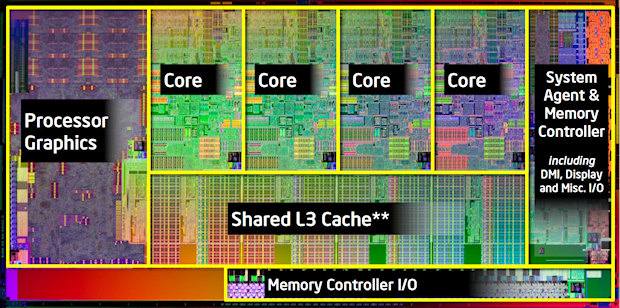
\includegraphics[width=9.5cm]{../../notes/03.multi/sandy}
\end{center}
\end{frame}

\begin{frame}\frametitle{The current supercomputer at NTNU}
Intel Sandy bridge E5-2670:
\vspace{.2cm}
\begin{itemize}
\item an octa-core chip (8 physical processing cores); 
\vspace{.2cm}
\item private L1 cache (32kB instruction+32kB data) 3 clocks; \\
      private L2 cache (256kB) 8 clocks; \\
      shared L3 cache (20MB) $\sim$ 30 clocks (could not find info); \\
      main memory (32GB) $\sim$ 150 clocks (could not find info).
\item FMA capable AVX unit, meaning 8 Flop/cycle, SSE 4.x.
\vspace{.2cm}
\item simultaneous multi-threading (SMT) - Intel calls this 'Hyperthreading': 
each processor core can handle two instruction streams at the same time.
Problem: Shared SIMD units
\end{itemize}
\end{frame}


\begin{frame}\frametitle{An SMP system (or a node): 2 E5-2670 chips}
\begin{itemize}
\item 2 physical processors + 32GB memory + I/O;
\item shared memory system.
\end{itemize}
\vspace{.2cm}
\begin{center}
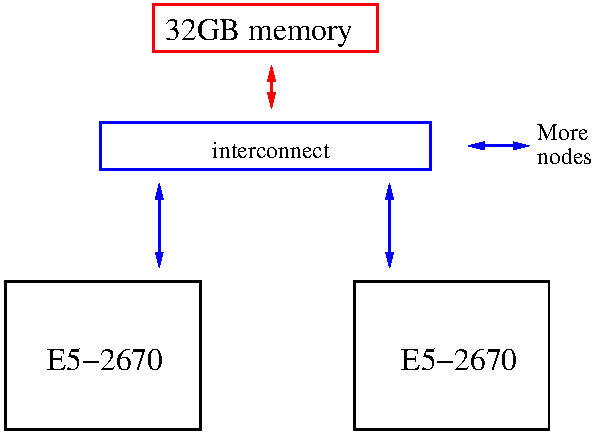
\includegraphics[width=7.5cm]{e5-2670}
\end{center}
\end{frame}

\begin{frame}\frametitle{Distributed SMPs}
\textcolor{red}{\texttt{vilje} @ NTNU}: 
\vspace{.2cm}
\begin{itemize}
  \item 1440 nodes or 23040 physical cores; 
  \item (16-core) shared memory within a single node; 
  \item distributed memory across nodes; 
  \item 394 TB storage.
  \item 8.6GB/s aggregated bandwidth.
  \end{itemize}
  \vspace{.5cm}
  \textcolor{blue}{Programming models}: 
  \begin{itemize}
  \item shared memory programming model (OpenMP) within a node;
  \item message passing (MPI) across nodes; 
  \vspace{.2cm}
  \item also possible: message passing within a single node; 
  \item also possible: both models within the same program.
  \end{itemize}
\end{frame}
\end{document}
